\documentclass[aspectratio=169]{beamer}

\usepackage{calc}
\usepackage{graphicx}

\graphicspath{{./images}}
\setbeamertemplate{navigation symbols}{}

\author{Chris Doble}
\date{}
\subtitle{Building a GPS receiver from scratch}
\title{Part 2: Correlation}
\usetheme{Madrid}

% Show the topics frame at the start of each section
\AtBeginSection[]
{
  \begin{frame}
    \frametitle{Topics}
    \tableofcontents[currentsection]
  \end{frame}
}

\begin{document}

\frame{\titlepage}

\begin{frame}
    \frametitle{Topics}

    \tableofcontents
\end{frame}

\section{Correlation}

\begin{frame}
    \frametitle{Positive correlation}

    \centering
    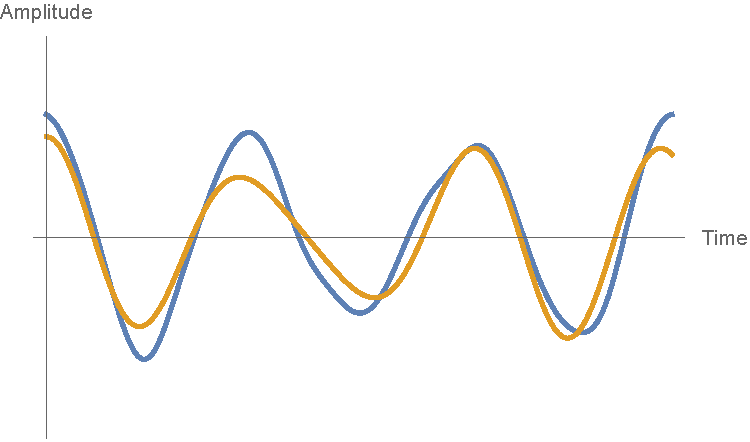
\includegraphics[width=\textwidth * 3 / 4]{1 positive.pdf}
\end{frame}

\begin{frame}
    \frametitle{Negative correlation}

    \centering
    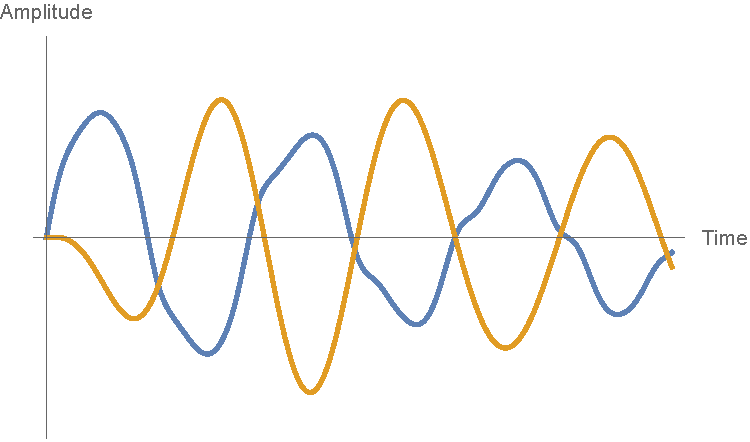
\includegraphics[width=\textwidth * 3 / 4]{2 negative.pdf}
\end{frame}

\begin{frame}
    \frametitle{Near-zero correlation}

    \centering
    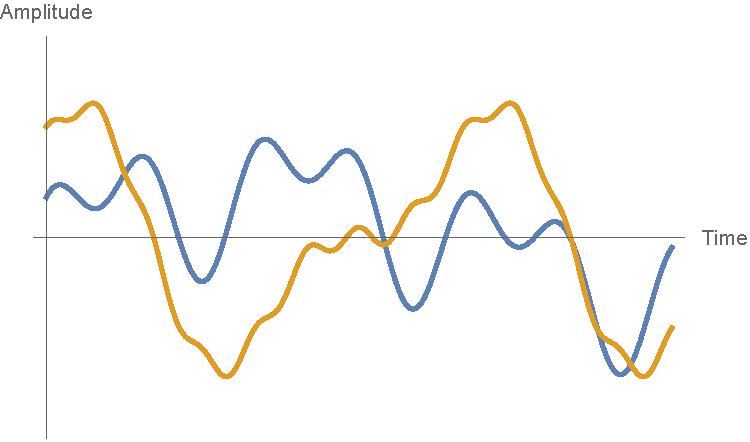
\includegraphics[width=\textwidth * 3 / 4]{3 zero.pdf}
\end{frame}

\begin{frame}
  \frametitle{Definition}

  The correlation of two signals $f(t)$ and $g(t)$ is defined as \[\int_{-\infty}^{+\infty} f(t) g(t) \,dt.\]
\end{frame}

\begin{frame}
  \frametitle{$f(t) \rightarrow 0$ as $|t| \rightarrow \infty$}

  \centering
  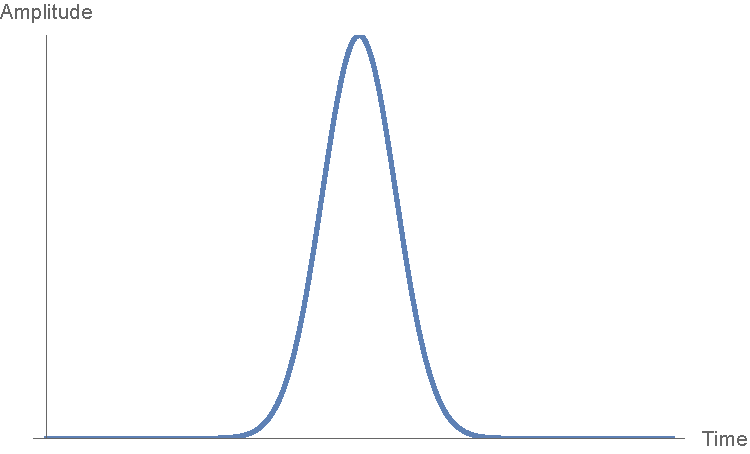
\includegraphics[width=\textwidth * 3 / 4]{4 square integrable.pdf}
\end{frame}

\begin{frame}
  \frametitle{Periodic signals}

  \centering
  \only<1>{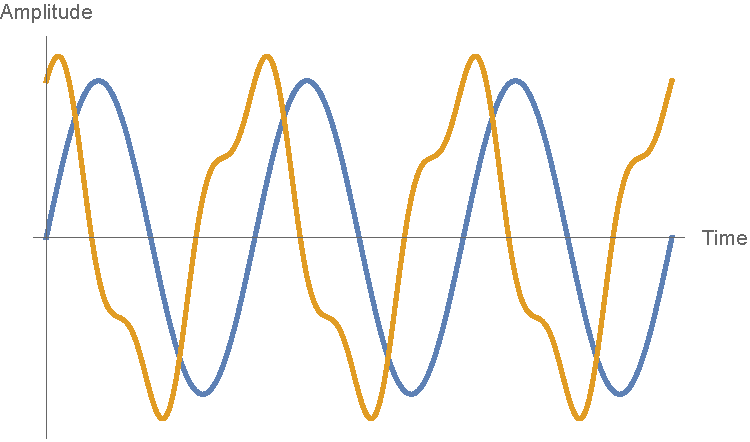
\includegraphics[width=\textwidth * 3 / 4]{5 periodic.pdf}}%
  \only<2>{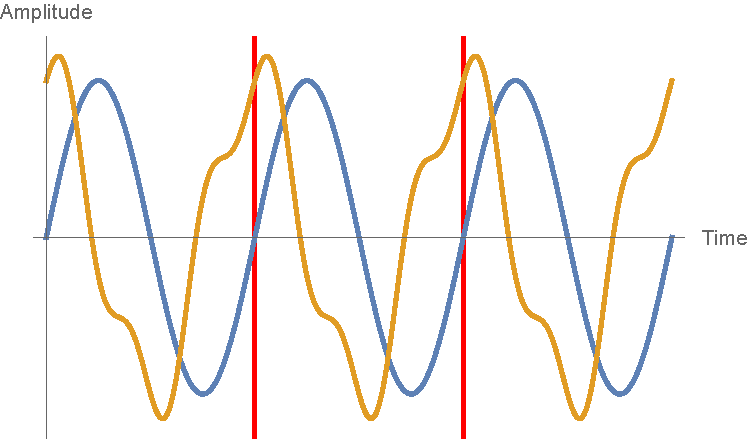
\includegraphics[width=\textwidth * 3 / 4]{6 periodic with bounds.pdf}}
\end{frame}

\begin{frame}
  \frametitle{Definition}
  
  The correlation of two periodic signals $f(t)$ and $g(t)$ is defined as \[\int_{t_0}^{t_0 + T} f(t) g(t) \,dt\] where $t_0$ is an arbitrary point in time and $T$ is their shared period.
\end{frame}

\begin{frame}
  \frametitle{Multiple periods}

  \centering
  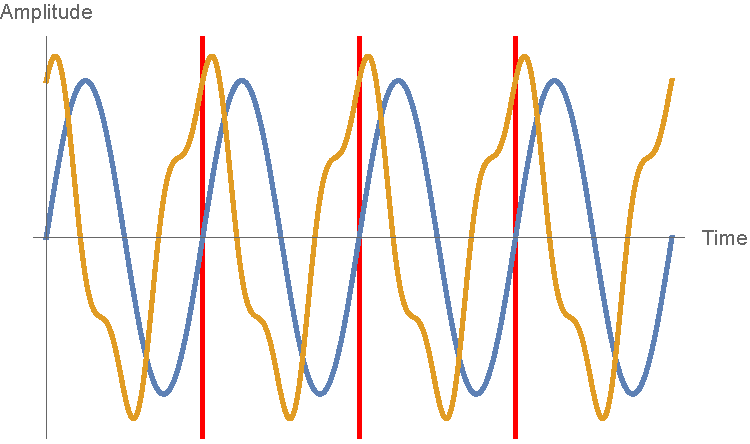
\includegraphics[width=\textwidth / 2]{7 multiple periods.pdf}

  \onslide<2->{\[\int_{t_0}^{t_0 + n T} f(t) g(t) \,d t = n \int_{t_0}^{t_0 + T} f(t) g(t) \,dt\]}
\end{frame}

\begin{frame}
  \frametitle{Definition vs. intuition}

  \[\int_{-\infty}^{+\infty} f(t) g(t) \,dt\]

  \begin{itemize}
    \item<2-> Same $\Rightarrow$ same signs $\Rightarrow$ positive products $\Rightarrow$ positive sum
    \item<3-> Opposite $\Rightarrow$ opposite signs $\Rightarrow$ negative products $\Rightarrow$ negative sum
    \item<4-> Not similar at all $\Rightarrow$ positive and negative products $\Rightarrow$ sums cancel
  \end{itemize}
\end{frame}

\section{Cross-correlation}

\section{Autocorrelation}

\begin{frame}
  \frametitle{Conclusion}

  \begin{itemize}
    \item<2-> Intuition of correlation
    
      \begin{itemize}
        \item Almost the same $\Rightarrow$ positive correlation
        
        \item Almost opposites $\Rightarrow$ negative correlation
        
        \item Not similar at all $\Rightarrow$ near-zero correlation
      \end{itemize}
        
    \item<3-> Definition of correlation
    
      \begin{itemize}
        \item $\int_{-\infty}^{+\infty} f(t) g(t) \,dt$
        
        \item $\int_{t_0}^{t_0 + T} f(t) g(t) \,dt$
      \end{itemize}
    
    \item<4-> Cross-correlation
    
      \begin{itemize}
        \item The correlation of two signals at different shifts
      \end{itemize}
    
    \item<5-> Autocorrelation
    
      \begin{itemize}
        \item The cross-correlation of a signal with itself
      \end{itemize}
  \end{itemize}
\end{frame}

\end{document}